\chapter{Experiments}

In this chapter we will describe practical experiments of our algorithm and their results. First, we will describe on which kind of data the experiments were made and how the experiments look like, and after that we will show diagrams describing how well our algorithm did during these experiments.

\section{Experiments description}

Experiments were made on two real datasets: \textit{DBLP}~--- graph, where vertices are the article authors and an edge between two vertices means that there is a common article between these two authors. Also, we made our experiments on \textit{Youtube} dataset~--- social graph where vertices are Youtube users and the edge between two vertices means mutual subscription.

For our experiments we've taken $50$ random queries without noise, $50$ queries with noise and $5$ queries with absolute noise, i.e. containing vertices that are have almost no common between each other. We will describe queries building more detailed below.

\begin{enumerate}
\item In first experiment we took $50$ random queries on graph, each of which contained vertices that highly correlated between each other. We built query by taking \textit{k-core} with quite big $k$ and then taking vertices from it randomly, however, taking into account that vertices shouldn't be far from each other. Here we should point out that Barbieri et al. \cite{Barbieri15} didn't take it into account and obtained size of components were almost $10$ times bigger than ours. As a result of the experiment, we were calculating average size of the community over $50$ experiments.

\item In the second experiment we took $50$ random queries on graph such that most of the query vertices highly correlated between each other and remaining vertices were noise, i.e. weakly correlated with other vertices. We built query by taking \textit{k-core} with quite big $k$ (i.e. the query generated by the first experiment) and adding few vertices from \textit{k-cores} with less $k$, i.e. the vertices being the noise. As a result we calculate the average size of the communite over $50$ experiments. 

\item In the third experiment to analyze the behaviour of our algorithm when the query is almost fully noisy, we choose several vertices from different \textit{k-cores} which are weakly connected and have almost no correlation betwen each other. This experiment has shown that on such queries our solutions build quite big subgraph, but it still filters noise quite good and the resulting size of the community is much smaller than in other algorithms.
\end{enumerate}

After each run of our algorithm, we also do answer validation~--- that the resulting subgraph contains most of the initial query vertices~--- at least $\max$($\frac{|Q|}{2}$, $|Q| \cdot \alpha - \epsilon$), where $\epsilon$ is a small number showing that after phase $2$ of our algorithm we could remove several weakly connected vertices on phase $3$. For our experiments we took $\epsilon = 4$.

\section{Results}

Here we will provide results of our experiments comparing our suggested algorith with Faloutsos \& Tong \cite{Faloutsos06}, Gionis et al. \cite{Gionis15} and Barbieri et al. \cite{Barbieri15}. For better vizualization we will provide several diagrams with small description. For each of datasets we will provide $6$ diagrams comparing density and size of the obtained subgraphs, and time taken to find these subgraphs (we don't take into account time taken for precalculations, only query time). We build diagrams for $2$ different types of queries~--- with and without noise respectively. In each diagram horizontal axes means different sizes of $|Q|$ (either $1$, $2$, $3$, $4$, $8$, $16$ or $32$) and vertical axes maans the density of the obtained subgraph, its size or time taken to find it.

\subsection{DBLP dataset}

\textit{DBLP} dataset contains $317080$ vertices and $1049866$ edges. It consists of article authors, where the edge between two authors means having common article between them.

\subsubsection{Queries without noise. Community density}

%\begin{figure}[!h]
%\caption{Queries without noise. Community density.}\label{dblp-density}
  \begin{center}
    \makebox[\textwidth]{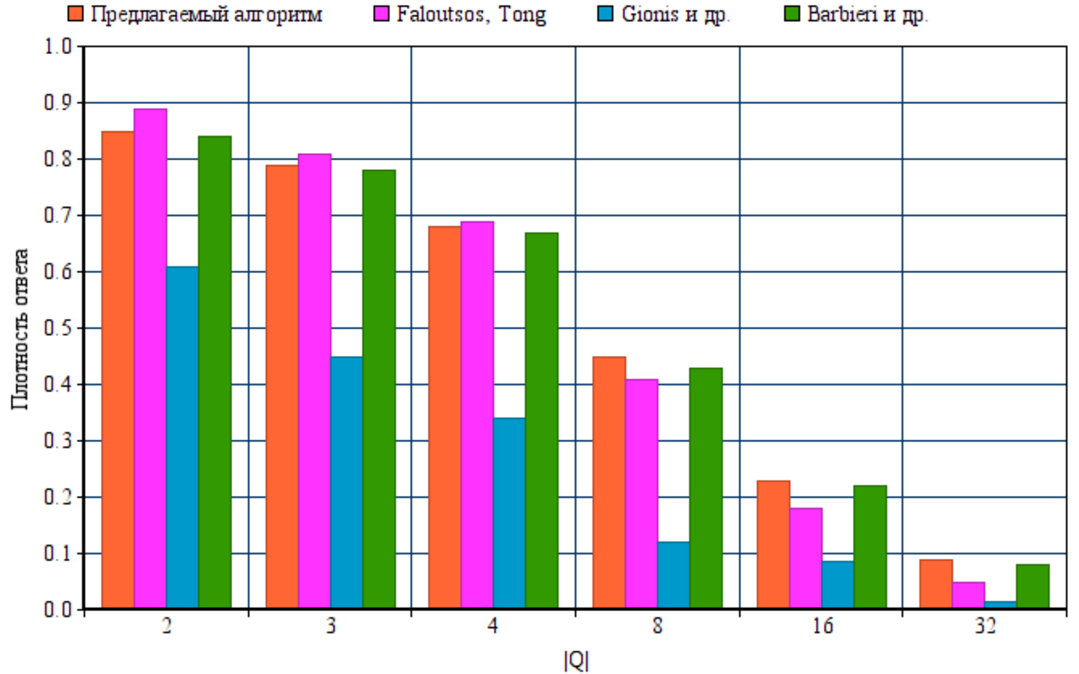
\includegraphics[scale=0.4]{pictures/results-dblp-density.png}}
  \end{center}
%\end{figure}

As you can see from the diagram, on random queries without noise the density of the community obtained by our alrogithm is a bit greater than the density of community obtained by Barbieri et al. \cite{Barbieri15}, what means that our algorithm is more optimal. Also, the density of our community is more on average than the density of Faloutsos \& Tong \cite{Faloutsos06} and much more than the density of Gionis et al. \cite{Gionis15}.

\subsubsection{Queries without noise. Community size}

%\begin{figure}[!h]
%\caption{Queries without noise. Community size.}\label{dblp-size}
  \begin{center}
    \makebox[\textwidth]{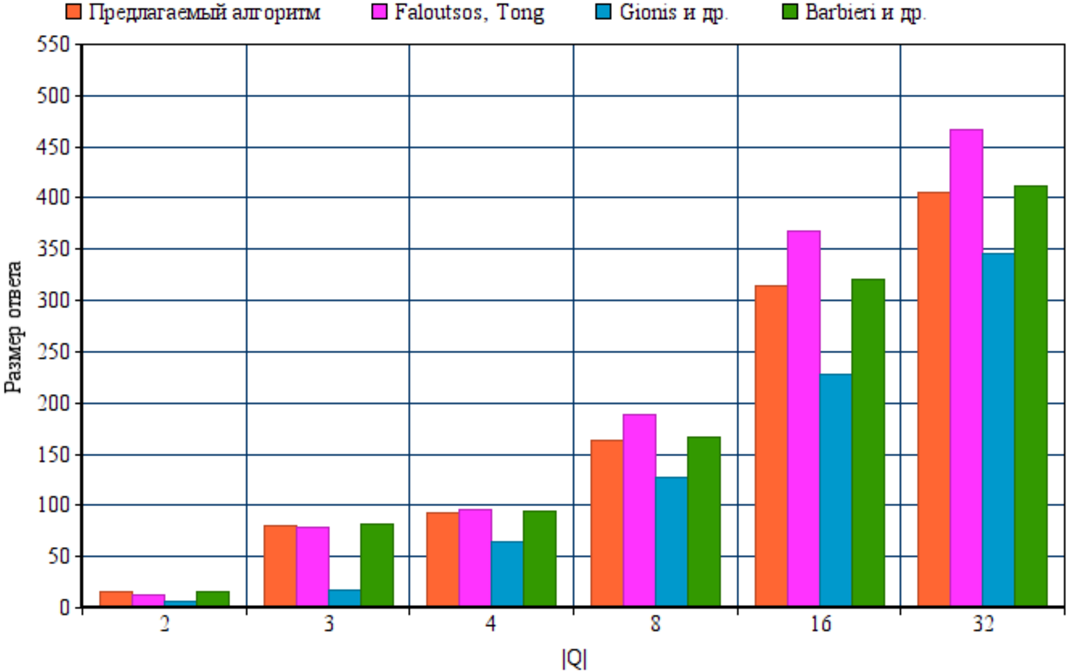
\includegraphics[scale=0.4]{pictures/results-dblp-size.png}}
  \end{center}
%\end{figure}

As you can see from the diagram, on random queries without noise the size of our community is a bit less than the size of community obtained by Barbieri et al. \cite{Barbieri15}, which is quite logical from the previous diagram. The size of our community is also less on average than the size of Faloutsos \& Tong \cite{Faloutsos06}, but greater than the size of Gionis et al. \cite{Gionis15}, but because our main goal is density, not the size, it's not an issue.

\subsubsection{Queries without noise. Work time}

%\begin{figure}[!h]
%\caption{Queries without noise. Work time.}\label{dblp-time}
  \begin{center}
    \makebox[\textwidth]{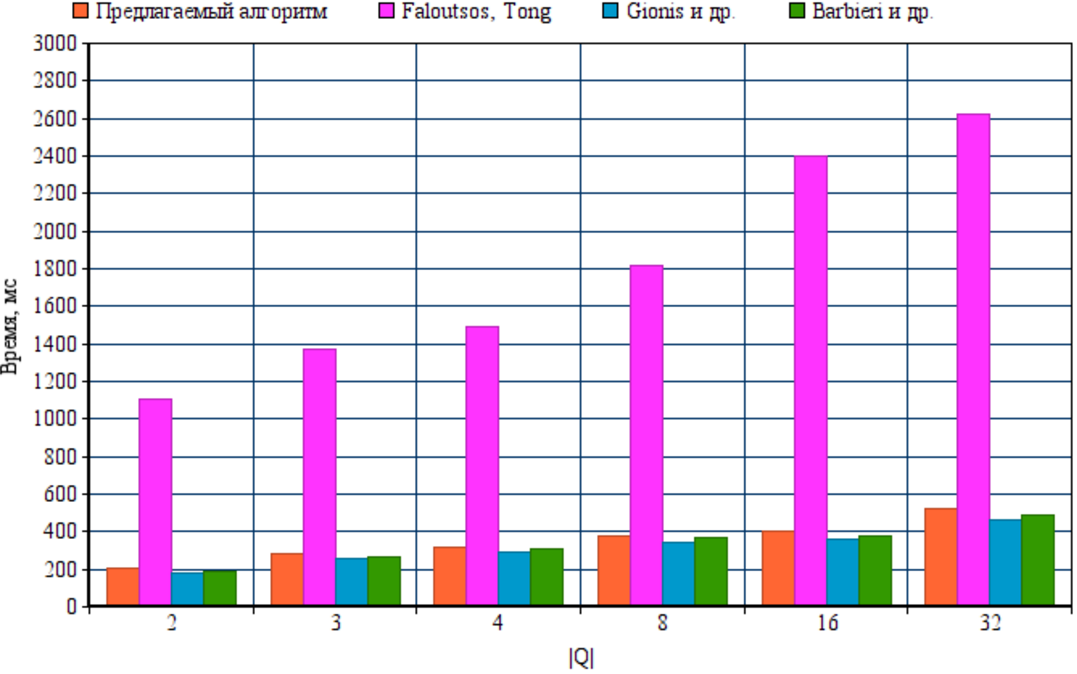
\includegraphics[scale=0.4]{pictures/results-dblp-time.png}}
  \end{center}
%\end{figure}

As you can see from the diagram, our algorithm takes a bit much time to process than Barbieri et al. \cite{Barbieri15}, but this loss is very minor. Faloutsos \& Tong \cite{Faloutsos06} takes much more time to find the answer and Gionis et al. \cite{Gionis15} works faster, but as we saw previously, it finds not dense subgraph, so it's ok for us.

\subsubsection{Queries with noise. Community density}

%\begin{figure}[!h]
%\caption{Queries with noise. Community density.}\label{dblp-density-noise}
  \begin{center}
    \makebox[\textwidth]{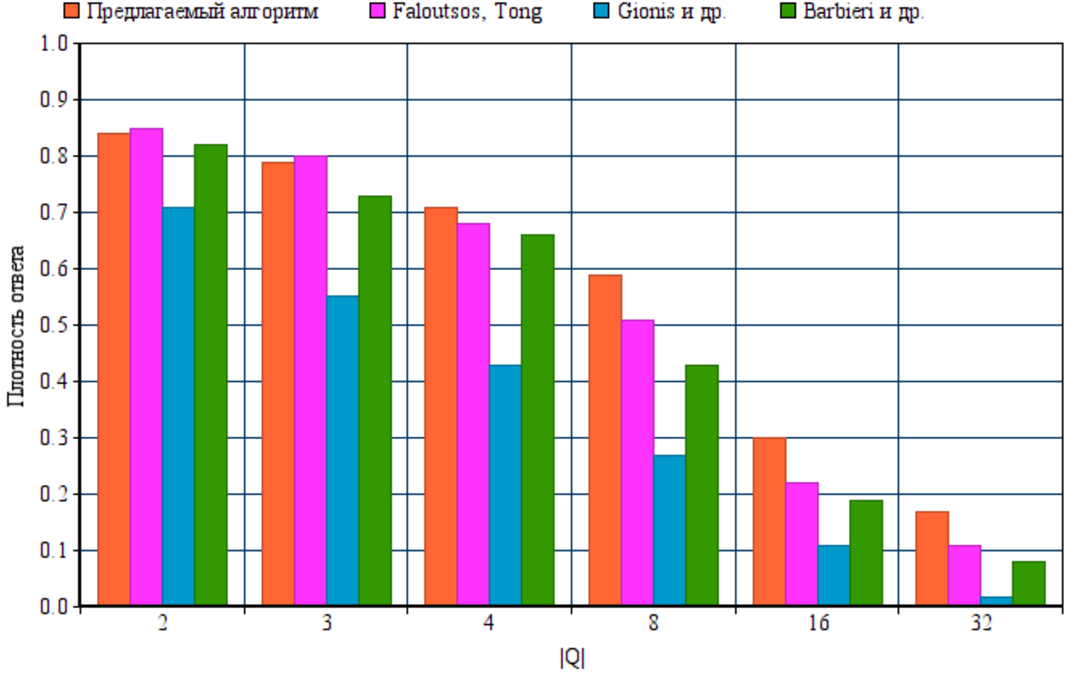
\includegraphics[scale=0.4]{pictures/results-dblp-density-noise.png}}
  \end{center}
%\end{figure}

If the query contains some noise, our algorithm starts working much more optimal comparing to other algorithmis. You can see it on the diagram above: on small $|Q|$ our win is not so big (because there is almost no noise), but on bigger $|Q|$ we are winning much more in terms of density and size.

\subsubsection{Queries with noise. Community size}

%\begin{figure}[!h]
%\caption{Queries with noise. Community size.}\label{dblp-size-noise}
  \begin{center}
    \makebox[\textwidth]{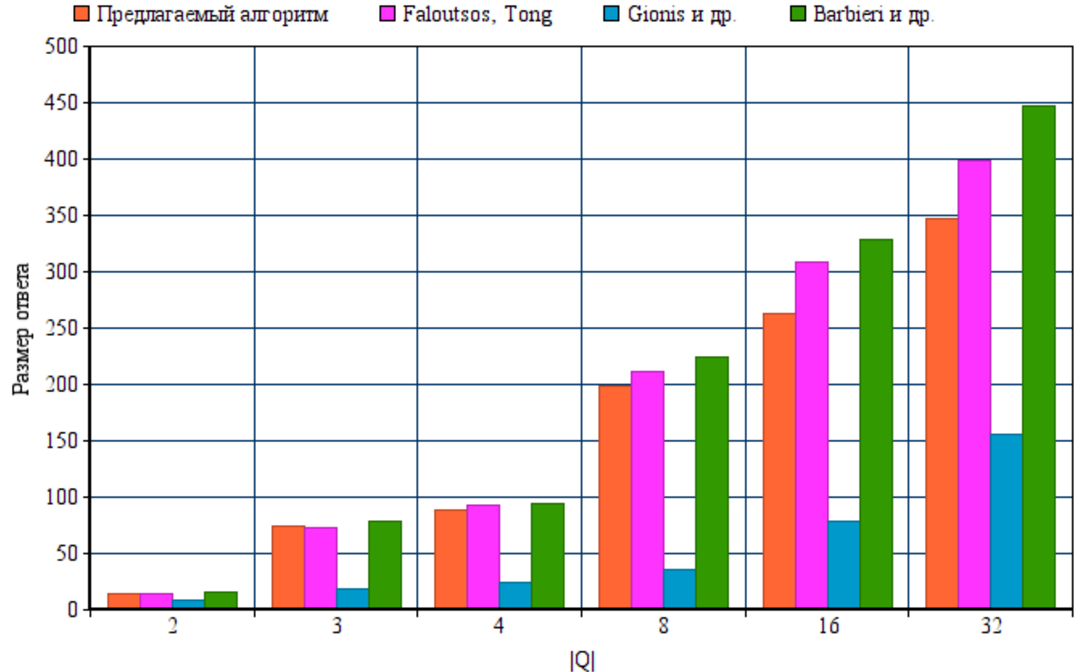
\includegraphics[scale=0.4]{pictures/results-dblp-size-noise.png}}
  \end{center}
%\end{figure}

As you can see from the diagram, if the noise exists, the size of our community is less than the size of community of other algorhtms (besides Gionis et al. \cite{Gionis15}, but it works worse in terms of density).

\subsubsection{Queries with noise. Work time}

%\begin{figure}[!h]
%\caption{Queries with noise. Work time.}\label{dblp-time-noise}
  \begin{center}
    \makebox[\textwidth]{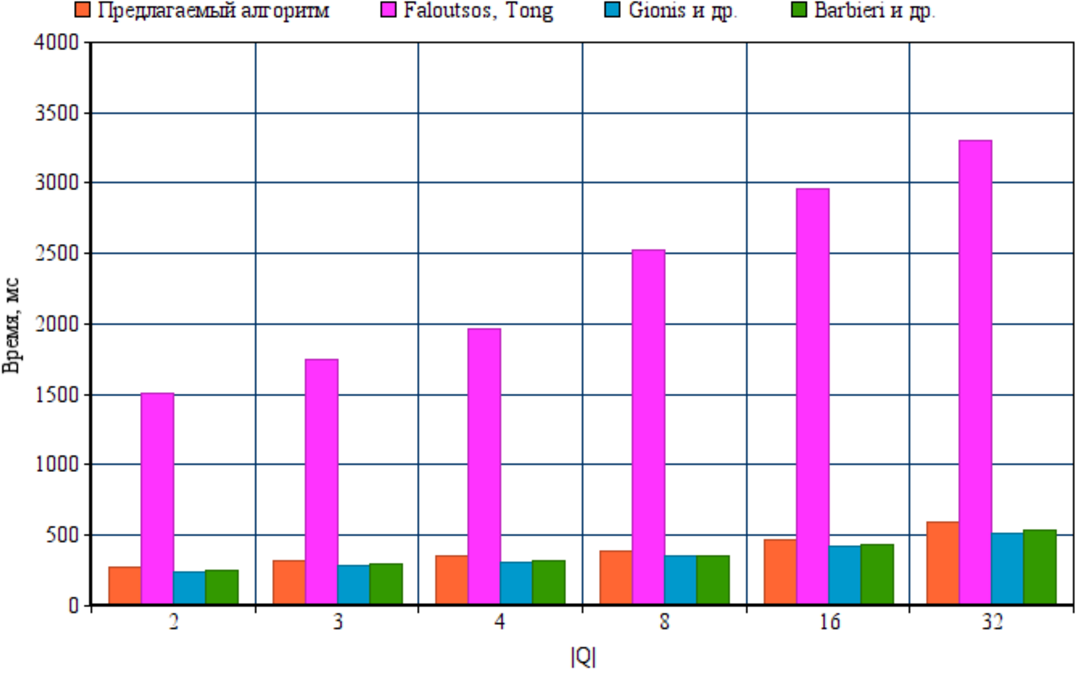
\includegraphics[scale=0.4]{pictures/results-dblp-time-noise.png}}
  \end{center}
%\end{figure}

Work time of our algorithm on queries with noise is a bit more than work time of Barbieri et al. \cite{Barbieri15}, however this loss is very minor and we won't take it into account.

\subsection{Youtube dataset}

\textit{Youtube} dataset contains $1134890$ and $2987624$ edges. This dataset consists of Youtube users and an edge between two vertices means that these two users have a common subscription, i.e. they are friends of each other.

Results for this dataset are pretty similar to the results for \textit{DBLP}, so we won't leave any comments for the diagrams and let you make all findings youself.

\subsubsection{Queries without noise. Community density}

%\begin{figure}[!h]
%\caption{Queries without noise. Community density.}\label{youtube-density}
  \begin{center}
    \makebox[\textwidth]{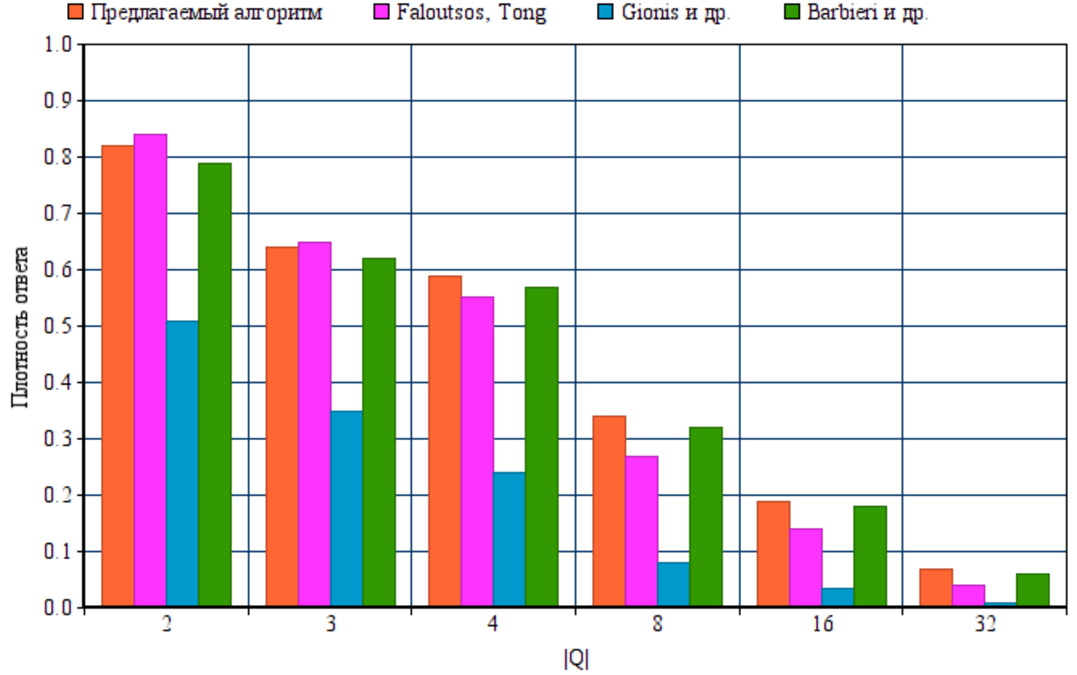
\includegraphics[scale=0.4]{pictures/results-youtube-density.png}}
  \end{center}
%\end{figure}

\subsubsection{Queries without noise. Community size}

%\begin{figure}[!h]
%\caption{Queries without noise. Community size.}\label{youtube-size}
  \begin{center}
    \makebox[\textwidth]{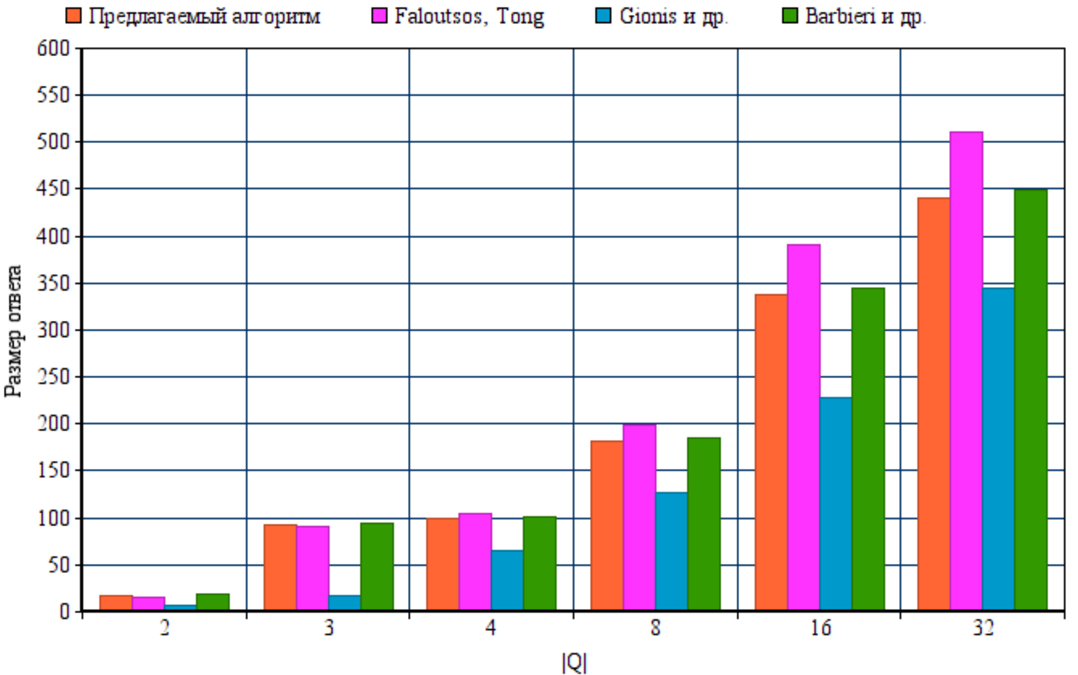
\includegraphics[scale=0.4]{pictures/results-youtube-size.png}}
  \end{center}
%\end{figure}
%\FloatBarrier

\subsubsection{Community without noise. Work time}

%\begin{figure}[!h]
%\caption{Community without noise. Work time.}\label{youtube-time}
  \begin{center}
    \makebox[\textwidth]{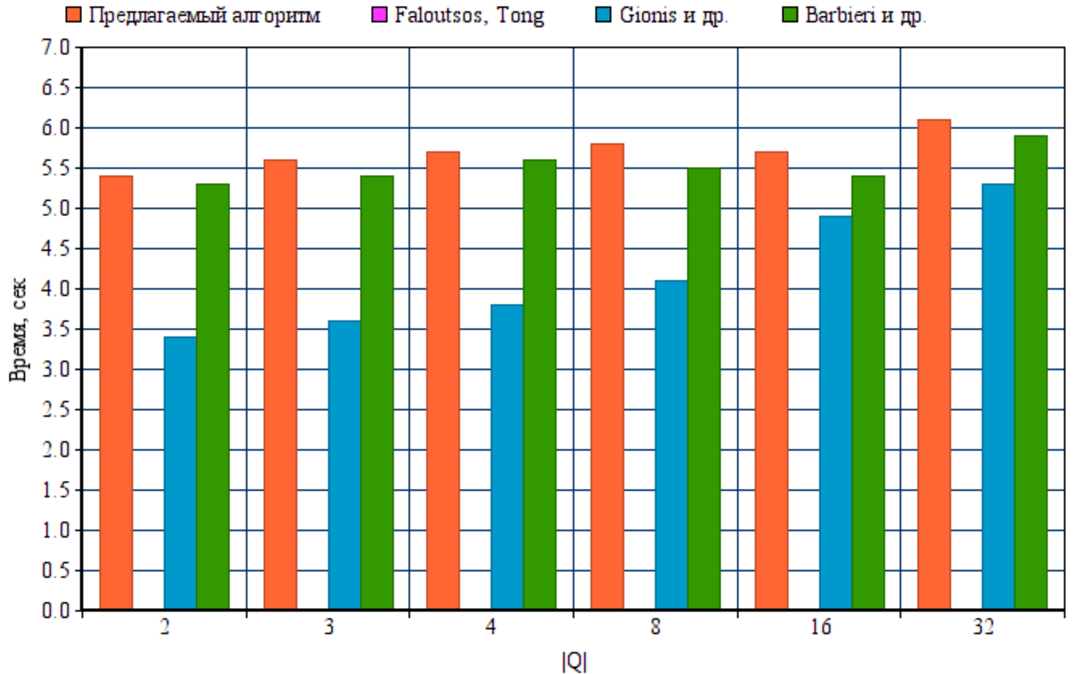
\includegraphics[scale=0.4]{pictures/results-youtube-time.png}}
  \end{center}
%\end{figure}

Here we can mention that Faloutsos \& Tong \cite{Faloutsos06} algorithm works takes too much time to proceed, so we removed it from diagram to avoid vizualization issues. Also, we should mention that work time is measured in seconds here because of the difference in dataset sizes comparing to \textit{DBLP}.

\subsubsection{Queries with noise. Community density}

%\begin{figure}[!h]
%\caption{Queries with noise. Community density.}\label{youtube-density-noise}
  \begin{center}
    \makebox[\textwidth]{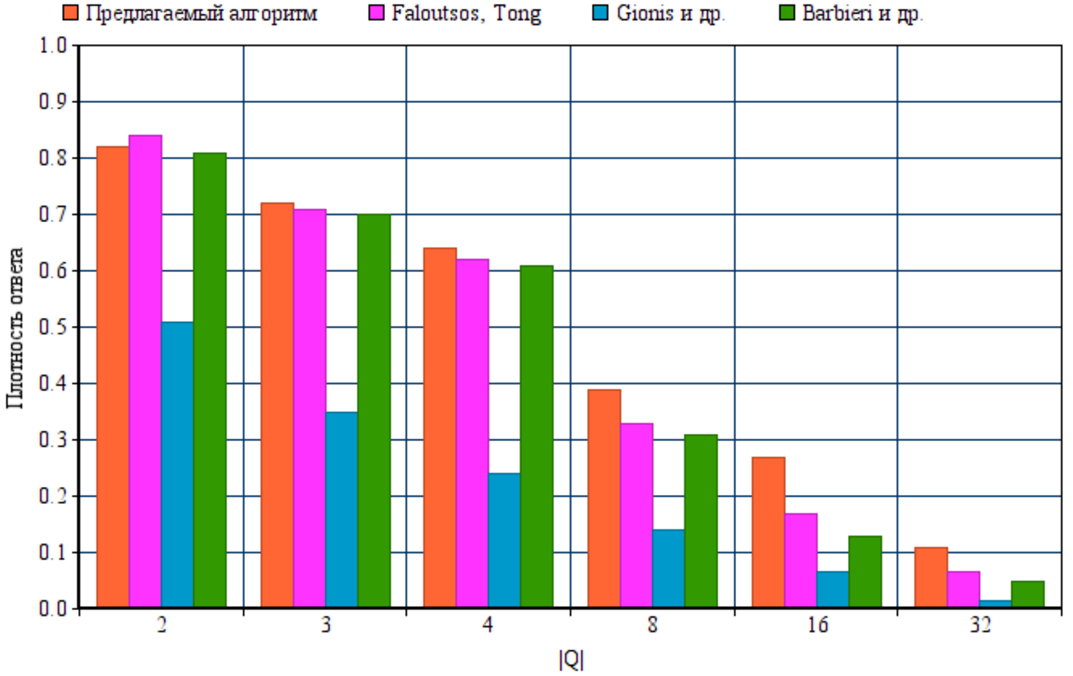
\includegraphics[scale=0.4]{pictures/results-youtube-density-noise.png}}
  \end{center}
%\end{figure}

\subsubsection{Queries with noise. Community size}

%\begin{figure}[!h]
%\caption{Queries with noise. Community size.}\label{youtube-size-noise}
  \begin{center}
    \makebox[\textwidth]{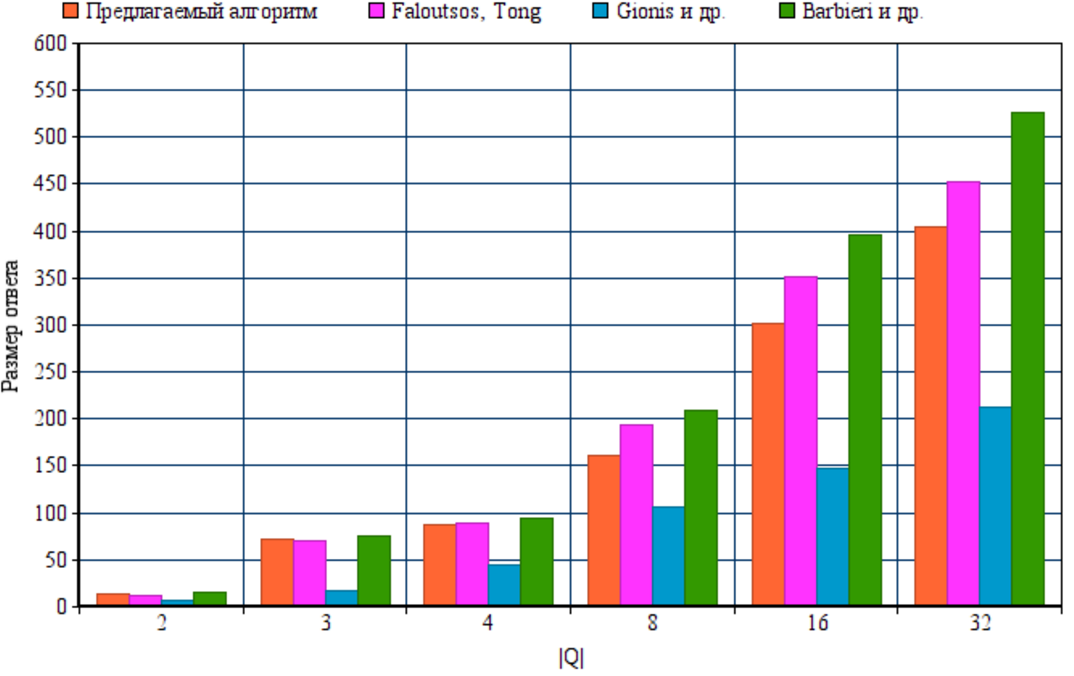
\includegraphics[scale=0.4]{pictures/results-youtube-size-noise.png}}
  \end{center}
%\end{figure}
%\FloatBarrier

\subsubsection{Queries with noise. Work time}

%\begin{figure}[!h]
%\caption{Queries with noise. Work time.}\label{youtube-time-noise}
  \begin{center}
    \makebox[\textwidth]{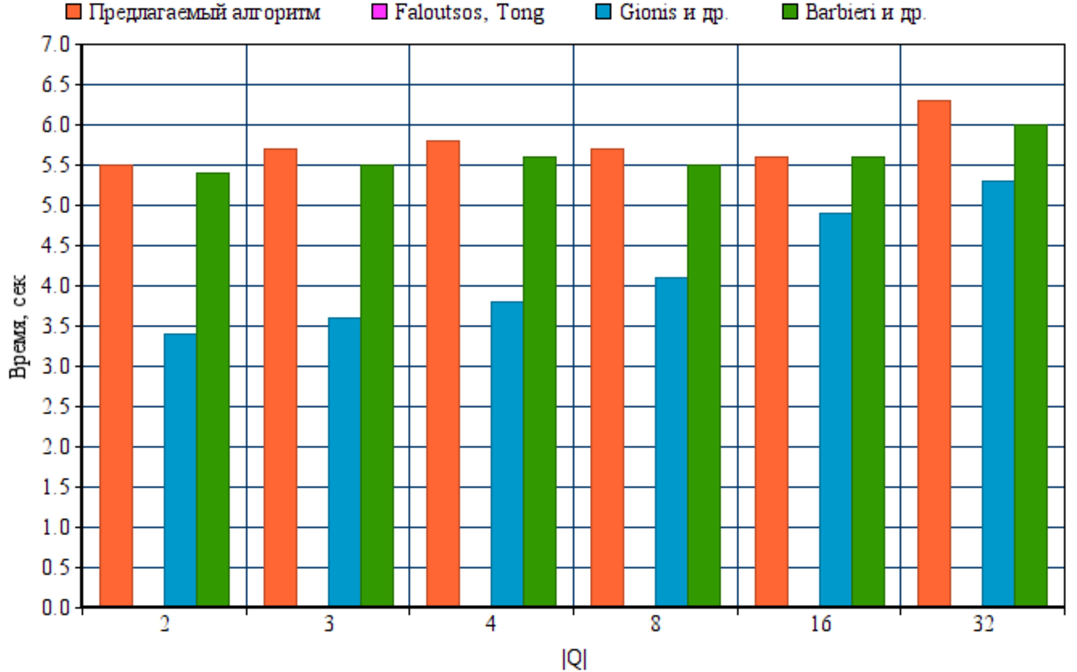
\includegraphics[scale=0.4]{pictures/results-youtube-time-noise.png}}
  \end{center}
%\end{figure}
%\FloatBarrier

The work time of Faloutsos \& Tong \cite{Faloutsos06} is not presented for the same reason.

\subsection{Final results}

Let's collect the results altogether. We collect these results in tables~\ref{results-dblp} and ~\ref{results-youtube}:

In these tables you can find how our solution compares to the other ones. In each cell we provide average result and maximal win respectively. For example, $18.1\%/54.6\%$ in <<density with noise>> cell means that in average we won $18.1\%$ by density, but the maximal win among all experiments was $54.6\%$. In size and work time $-4.7\%/-14.6\%$ means that our size is $4.7\%$ less in average and $14.6\%$ less on the best experiment.

\begin{table}[!h]
\centering
\caption{DBLP dataset}\label{results-dblp}
  \begin{tabular}{| l | l | l | p{4cm} |}
  \hline
  -- & Faloutsos \& Tong & Gionis et al. & Barbieri et al. \\\hline
  Density         & +18.2\% / +80.0\% & +200.6\% / +542.9\% & 4.2\%   / +12.5\%  \\\hline
  Size            & -4.5\%  / -14.4\% & +97.4\%  / +17.7\%  & -2.9\%  / -6.25\%  \\\hline
  Time            & -80.3\% / -83.3\% & +11.7\%  / +7.7\%   & +5.2\%  / +2.7\%   \\\hline
  Density (noise) & +18.1\% / +54.6\% & +210.4\% / +844.4\% & +37.6\% / +112.5\% \\\hline
  Size (noise)    & -4.7\%  / -14.6\% & +247.9\% / +87.5\%  & -11.6\% / -22.4\%  \\\hline
  Time (noise)    & -82.8\% / -84.6\% & +12.1\%  / +10.3\%  & +8.4\%  / +6.6\%   \\\hline
  \end{tabular}
\end{table}
\FloatBarrier

\begin{table}[!h]
\centering
\caption{Youtube dataset}\label{results-youtube}
  \begin{tabular}{| l | l | l | p{3.8cm} |}
  \hline
  -- & Faloutsos \& Tong & Gionis et al. & Barbieri et al. \\\hline
  Density         & +23.3\%  / +75.0\%  & +305.4\% / +775.0\% & +6.5\%  / +16.7\%  \\\hline
  Size            & -4.6\%   / -13.7\%  & +123.3\% / +27.9\%  & -2.6\%  / -5.3\%   \\\hline
  Time            & -320.8\% / -325.1\% & +39.6\%  / +15.1\%  & +3.6\%  / +1.8\%   \\\hline
  Density (noise) & +24.7\%  / +69.2\%  & +252.1\% / +685.7\% & +45.3\% / +129.2\% \\\hline
  Size (noise)    & -4.3\%   / -17.0\%  & +223.3\% / +27.8\%  & -14.8\% / -23.7\%  \\\hline
  Time (noise)    & -323.4\% / -331.1\% & +40.8\%  / +14.2\%  & +2.9\%  / +0.0\%   \\\hline
  \end{tabular}
\end{table}
\FloatBarrier

We're also worried about the following thing~--- is it possible that on queries without any noise our algorithm will throw away some vertices thinking that it's a noise? Our experiments showed that it is possible, but actually because the query doesn't contain any noise, its vertices are densely connected and our algorithm will find almost no noise, only few vertices. Results have shown that we throw away only $2-3$ vertices from $Q$ (if $|Q| = 32$), which is quite normal behaviour.
